\pdfoutput=1
\documentclass[conference]{IEEEtran}
\IEEEoverridecommandlockouts
% The preceding line is only needed to identify funding in the first footnote. If that is unneeded, please comment it out.
\PassOptionsToPackage{table, x11names, dvipsnames, svgnames}{xcolor}
\usepackage{cite}
\usepackage{bbm}
\usepackage{amsmath,amssymb,amsfonts}
\usepackage{algorithmic}
\usepackage{graphicx}
\usepackage{textcomp}
\usepackage{xcolor}
\usepackage[english]{babel}
\usepackage[acronym,nonumberlist]{glossaries}
\usepackage{glossaries-prefix}
\usepackage{pgfplots}
\pgfplotsset{compat=1.17}
\usepgfplotslibrary{fillbetween}
\usepackage{amssymb}
\usepackage{import}
\usepackage{bm}
\usepackage{siunitx}
% conflicts with IEEE format
% \usepackage{subcaption}
\usepackage{multirow}
\usepackage[]{yquant}
\usepackage{hyperref}
\hypersetup{%
%colorlinks=true, 
linktocpage=true, 
colorlinks=false,
pdfborder={0 0 0}, %pdfstartpage=3, pdfstartview=FitV,%
breaklinks=true, pdfpagemode=UseNone, pageanchor=true, pdfpagemode=UseOutlines,%
plainpages=false, bookmarksnumbered, bookmarksopen=true, bookmarksopenlevel=1,%
hypertexnames=true, pdfhighlight=/O,%hyperfootnotes=true,%nesting=true,%frenchlinks,%
pdftitle={An Empirical Comparison of Optimizers for
Quantum Machine Learning with SPSA-based
Gradients},%
pdfauthor={Maniraman Periyasam},%
pdfsubject={QML},%
pdfkeywords={},%
pdfcreator={pdfLaTeX},%
pdfproducer={LaTeX with hyperref}%
}

% for reviewers reply
%\usepackage{rebuttal}

% For inline enumerations
\usepackage[inline]{enumitem}

\usepackage[capitalise]{cleveref}

%\makenoidxglossaries
\newacronym[shortplural=GMMs]{GMM}{GMM}{Gaussian mixture model}
\newacronym[shortplural=HMMs]{HMM}{HMM}{hidden Markov model}
\newacronym[shortplural=DNNs]{DNN}{DNN}{deep neural network}
\newacronym[shortplural=SVDs]{SVD}{SVD}{singular value decomposition}
\newacronym[
    prefixfirst={a\ },% prefix used on first use
    prefix={an\ }% prefix used on subsequent use
]{MCTS}{MCTS}{Monte Carlo tree search}
\newacronym[prefixfirst={a\ },prefix={an\ }]{MDP}{MDP}{Markov decision process}
\newacronym{CMDP}{CMDP}{constrained Markov decision process}
\newacronym{RL}{RL}{reinforcement learning}
\newacronym[shortplural=DTs]{DT}{DT}{decision tree}
\newacronym{SMT}{SMT}{satisfiability modulo theories}
\newacronym{IL}{IL}{Imitation Learning}
\newacronym[shortplural=CNNs]{CNN}{CNN}{convolutional neural network}
\newacronym[shortplural=DQNs]{DQN}{DQN}{deep Q-network}
\newacronym{AI}{AI}{artificial intelligence}
\newacronym{PPO}{PPO}{proximal policy optimization}
\newacronym{ML}{ML}{machine learning}
\newacronym{QML}{QML}{quantum machine learning}
\newacronym{NISQ}{NISQ}{noisy intermediate scale quantum}
\newacronym{QC}{QC}{quantum circuit}
\newacronym{VQC}{VQC}{variational quantum circuit}
\newacronym{VQA}{VQA}{variational quantum algorithm}
\newacronym{MNIST}{MNIST}{modified national institute of standards and technology}
\newacronym{FIM}{FIM}{Fisher information matrix}
\newacronym{IDU}{IDU}{incremental data-uploading}
\newacronym{DRU}{DRU}{data re-uploading}
\newacronym{QRL}{QRL}{quantum reinforcement learning}
\newacronym{SPSA}{SPSA}{simultaneous perturbation stochastic approximation}
\newacronym{SGD}{SGD}{stochastic gradient descent}
\newacronym{QEM}{QEM}{quantum error mitigation}

%-- layout -----------------------------
\renewcommand{\floatpagefraction}{.9}    % default: .5
\renewcommand{\topfraction}{0.99}         % 90% of page top can be a float (Standard 0.7)
\setcounter{topnumber}{15}
\setcounter{dbltopnumber}{15}
\renewcommand{\bottomfraction}{0.99}      % 90% of page bottom can be a float (Standard 0.3)
\setcounter{bottomnumber}{15}
\setcounter{totalnumber}{99}
\renewcommand{\textfraction}{0.01}        % only 10% of page must to be text (Standard 0.2)
%
\clubpenalty=10000
\widowpenalty=10000
\linepenalty=10
\hyphenpenalty=50
\pretolerance=100
\tolerance=1000
\hfuzz=2pt
\vfuzz=1pt
\exhyphenpenalty=50
%\allowdisplaybreaks

% \usepackage{lineno,todonotes}
% \newcommand{\todoALL}[1]{\todo[color=orange!20,inline]{@ALL: #1}}
% \newcommand{\todoMani}[1]{\todo[color=blue!20,inline]{@Mani: #1}}
% \newcommand{\todoNico}[1]{\todo[color=red!20,inline]{@Nico: #1}}
% \newcommand{\todoAxel}[1]{\todo[color=green!20,inline]{@Axel: #1}}
% \newcommand{\todoChris}[1]{\todo[color=magenta!20]{@Chris: #1}}
% \newcommand{\todoChristian}[1]{\todo[color=cyan!20,inline]{@Christian: #1}}
% \newcommand{\todoALLIn}[1]{\todo[inline,color=orange!20]{@ALL: #1}}


\begin{document}

%\onecolumn
%\input{reviewReply}

%\setcounter{figure}{0}
%\setcounter{table}{0}
%\twocolumn


\title{An Empirical Comparison of Optimizers for Quantum Machine Learning with SPSA-based Gradients
%{\footnotesize \textsuperscript{*}Note: Sub-titles are not captured in Xplore and should not be used}
\thanks{

* These authors contributed equally (name order randomised). \\
The research is supported by the Bavarian Ministry of Economic Affairs, Regional Development and Energy with funds from the Hightech Agenda Bayern via the project BayQS.\\
email address for correspondence: 
maniraman.periyasamy@iis.fraunhofer.de}
}

\author{
%
\IEEEauthorblockN{Marco Wiedmann*, Marc Hölle*, Maniraman Periyasamy*, Nico Meyer, 
Christian Ufrecht, Daniel D.\ Scherer, \\ Axel Plinge, and Christopher Mutschler}
\IEEEauthorblockA{\textit{Fraunhofer IIS, Fraunhofer Institute for Integrated Circuits IIS},
Nuremberg, Germany \\\vspace{1mm}}
}



\maketitle

\begin{abstract}
\Glspl{VQA} have attracted a lot of attention from the quantum computing community for the last few years. Their hybrid quantum-classical nature with relatively shallow quantum circuits makes them a promising platform for demonstrating the capabilities of \gls{NISQ} devices. Although the classical machine learning community focuses on gradient-based parameter optimization, finding near-exact gradients for \glspl{VQC} with the parameter-shift rule introduces a large sampling overhead. Therefore, gradient-free optimizers have gained popularity in quantum machine learning circles. Among the most promising candidates is the \gls{SPSA} algorithm, due to its low computational cost and inherent noise resilience. We introduce a novel approach that uses the approximated gradient from \gls{SPSA} in combination with state-of-the-art gradient-based classical optimizers. We demonstrate numerically that this outperforms both standard \gls{SPSA} and the parameter-shift rule in terms of convergence rate and absolute error in simple regression tasks. The improvement of our novel approach over \gls{SPSA} with \gls{SGD} is even amplified when shot- and hardware-noise are taken into account. We also demonstrate that error mitigation does not significantly affect our results.
\end{abstract}

\begin{IEEEkeywords}
variational quantum computing, quantum error mitigation, SPSA, gradient free optimization, classical optimizers, quantum regression.
\end{IEEEkeywords}

\glsresetall
%%%%%%%%%%%%%%%%%%%%%%%%%%%%%%%%%%%%%%%%%%%%%
%%%%% Sections %%%%%%%%%%%%%%%%%%%%%%%%%%%%%%
3D human pose estimation has ubiquitous applications in sport analysis, human-computer interaction, and fitness and dance teaching. While there has been remarkable progress in 3D pose estimation from a monocular image or video~\cite{hmrKanazawa17, Moon_2020_ECCV_I2L-MeshNet, kolotouros2019spin, kocabas2019vibe, xiang2019monocular}, inevitable challenges such as the depth ambiguity and the self-occlusion are still unsolved. 



\begin{figure}
     \centering
     \begin{subfigure}[h]{0.23\textwidth}
         \centering
         \includegraphics[width=\textwidth]{figures/cover/image-comp.jpg}
         \caption*{Input image}
     \end{subfigure}
     \begin{subfigure}[h]{0.23\textwidth}
         \centering
         \includegraphics[width=\textwidth]{figures/cover/smplify-comp.jpg}
         \caption*{SMPLify-X~\cite{SMPL-X:2019}}
     \end{subfigure}
     \vspace*{0.2cm}
     \begin{subfigure}[h]{0.45\textwidth}
         \centering
         \includegraphics[width=0.98\linewidth, trim=25 50 25 50]{figures/cover/scene_cover_green-comp.png}
         \caption*{3D visualization of our (left) and SMPLify-X (right) results}
     \end{subfigure}
     \vspace*{-0.2cm}
     \caption{While the state-of-the-art single-view 3D pose estimator~\cite{SMPL-X:2019} yields a small reprojection error, the recovered 3D poses may be erroneous due to the depth ambiguity. We make use of the mirror in the image to resolve the ambiguity and reconstruct more accurate human pose as well as the mirror geometry.}
     \vspace*{-0.5cm}
    \label{fig:demo1}
\end{figure}



In many scenes like dancing rooms and gyms, people are often in front of a mirror. In this case, we are able to see the person and his/her mirror image simultaneously. The mirror image actually provides an additional virtual view of the person, which can resolve the single-view depth ambiguity if the mirror is properly placed. Moreover, unseen part of the person can also be observed from the mirror image, so that the occlusion problem can be alleviated. 


In this paper, we investigate the feasibility of leveraging such mirror images to improve the accuracy of 3D human pose estimation. We develop an optimization-based framework with mirror symmetry constraints that are applicable without knowing the mirror geometry and camera parameters. We also provide a method to utilize the properties of vanishing points to recover the mirror normal along with the camera parameters, so that an additional mirror normal constraint can be imposed to further improve the human pose estimation accuracy. The effectiveness of our framework is validated on a new dataset for this new task with 3D pose ground-truth provided by a multi-view camera system. 


An important application of the proposed approach is to generate pseudo ground-truth annotations to train existing 3D pose estimators. To this end, we collect a large-scale set of Internet images that contain people and mirrors and generate 3D pose annotations with the proposed optimization method. The dataset is named Mirrored-Human.  
Compared with existing 3D human pose datasets~\cite{h36m_pami,mono-3dhp2017,vonMarcard2018} that are captured with very few subjects and background scenes, Mirrored-Human has a significantly larger diversity in human poses, appearances and backgrounds, as shown in Fig.~\ref{fig:dataset}. The experiments show that, by combining Mirrored-Human with existing datasets as training data, both accuracy and generalizability of existing 3D pose estimation methods can be significantly improved for both single-person and multi-person cases.   

In summary, we make the following contributions:
\begin{itemize}
    \item We introduce a new task of reconstructing  human pose from a single image in which we can see the person and the person's mirror image. 
    \item We develop a novel optimization-based framework with mirror symmetry constraints to solve this new task, as well as a method to recover mirror geometry from a single image.
    \item We collect a large-scale dataset named Mirrored-Human from the Internet, provide our reconstructed 3D poses as pseudo ground-truth, and show that training on this new dataset can improve the performance of existing 3D human pose estimators. 
\end{itemize}







\section{Theoretical Background}
\label{sec:Theory}
To give theoretical background, we start by introducing \glspl{VQC} and continue by presenting the parameter-shift rule and SPSA. Furthermore, we give a detailed list of the optimizers we examine in this work and close with a look at \gls{QEM}.

\subsection{Variational Quantum Circuits}
\label{sec:vqc}
A \gls{VQC} can be formally described as a sequence of parameterized gates $U(\bm{x}, \bm{\theta})$, that prepares a quantum state depending on the initial state $| \psi_0 \rangle$, input $\bm{x}$ and variational parameters $\bm{\theta}$. The output is obtained by computing the expectation value of an observable $A$ \cite{Schuld19}
\begin{equation}
\label{eq:expectation_value}
    f(\bm{x}, \bm{\theta}) := \langle \psi_0 | U^\dagger(\bm{x}, \bm{\theta}) A U(\bm{x}, \bm{\theta}) | \psi_0 \rangle .
\end{equation}
In the following, we will drop the dependency on the input $\bm{x}$ to facilitate the notation.
During the training of this circuit, we want to minimize a loss function $L(f(\bm{\theta}), y)$ with respect to some target values $y$ by tuning the circuit parameters $\bm{\theta}$. For example, this can be realized by iterative gradient descent steps:

\begin{equation}
\label{eq:gradient_step}
    \hat{\bm{\theta}}^{k+1} = \hat{\bm{\theta}}^k - \alpha^k \nabla L(\hat{\bm{\theta}}^k), %\overset{\tiny a)}{=} \hat{\bm{\theta}}^k - \alpha^k \nabla f(\hat{\bm{\theta}}^k)
\end{equation}
where $\hat{\bm{\theta}}^k$ denotes the updated parameter vector, $\alpha^k$ the learning rate and $\nabla L(\hat{\bm{\theta}}^k)$ the gradient at iteration $k$.  
%Without loss of generality we set $L(f(\bm{\theta}), y) = f(\bm{\theta})$ in a), where for more general cases the chain rule can be applied.

\subsection{Gradient Computation}
\label{sec:gradient_estimation}
In order to determine this gradient, we need to compute partial derivatives $\partial_{\theta_i} f(\bm{\theta})$ of the expectation in \cref{eq:expectation_value}, which arise due to the chain rule. Since the classical computational cost of computing the unitary $U$ increases exponentially for larger circuits, it is necessary to obtain gradients directly from the quantum hardware.
%This is where the parameter-shift rule is typically employed to yield estimates of these analytical partial derivatives. %from two estimations of $f(\bm{\theta})$ with shifted parameters. %analytical partial derivatives by computing $f(\bm{\theta})$ twice with shifted parameter $\theta_i$.

%Approaches like automatic gradient computation through backpropagation, as is common in Neural Networks, have no immediate analog in quantum computations, since measurements are irreversible.

\subsubsection{Parameter-shift rule}
%For the introduction of the parameter-shift rule it is sufficient to consider a single qubit parameterized gate $U_G(\theta)$ with a Hermitian generator $G$ with two distinct eigenvalues $e_0$ and $e_1$ and a real valued constant $a$ as:
\iffalse
Following the derivation of the partial derivative $\partial_{\theta_i} f(\bm{\theta})$ in \cite{Schuld19} and \cite{Crooks19}, we can decompose the unitary $U(\bm{\theta})$ into a product $U(\bm{\theta}) = V\mathcal{G}(\theta_i)W$ and regard all other parameters as constant: %, for which the product rule of calculus holds: %into the state $|\psi' \rangle = $ and following ones into the observable $A$.
\begin{equation}
\label{eq:partial_f}
    \partial_{\theta_i} f(\bm{\theta}) = \partial_{\theta_i} \langle \psi' | \mathcal{G}^\dagger(\theta_i) B \mathcal{G}({\theta_i}) | \psi' \rangle
\end{equation}
Where $B = V^\dagger A V$ and $| \psi' \rangle = W | \psi \rangle $.

If we only consider gates $\mathcal{G}(\theta_i)$ with a Hermitian generator $G$ that has two distinct eigenvalues $e_0$ and $e_1$ we can write:
\begin{equation}
    \mathcal{G}(\theta_i) = e^{-ia\theta_i G} = I \mathrm{cos}(r \theta_i) - i \frac{a}{r} G \mathrm{sin}(r \theta_i)
\end{equation}
with $r = \frac{a}{2}(e_1 - e_0)$ and \(I\) the identity operator. From this follows:
\begin{equation}
\label{eq:special_case}
    \mathcal{G}(\pm \frac{\pi}{4r}) = \frac{1}{\sqrt{2}}(I \mp i \frac{a}{r}G)
\end{equation}
We observe that:
\begin{equation}
\label{eq:partial_G}
    \partial_{\theta_i} \mathcal{G}(\theta_i) = -iaGe^{-ia\theta_iG}
\end{equation}
After substituting \eqref{eq:partial_G} and \eqref{eq:special_case} into \cref{eq:partial_f} and rearranging we get the parameter-shift rule:
\begin{equation}
\label{eq:param_shift}
    \partial_{\theta_i} f(\bm{\theta}) = r \left[ f(\bm{\theta} + \bm{s}) -  f(\bm{\theta} - \bm{s})\right]
\end{equation}
With the components of shift $\bm{s}$ being $s_i = \frac{\pi}{4r}$ and $s_j = 0 \; \forall \; j \neq i$.
%For a detailed derivation we refer to \cite{Schuld19}.
\fi

%If we only consider gates with a Hermitian generator that has two distinct eigenvalues $e_0$ and $e_1$ the parameter-shift rule states
The parameter-shift rule enables the computation of exact partial derivatives of \cref{eq:expectation_value} from two expectation values per parameter.
Following refs. \cite{Schuld19} and \cite{Crooks19}, in order to compute the partial derivative \(\partial_{\theta_i}f(\bm{\theta})\) with respect to a single parameter \(\theta_i\), we factor the circuit unitary $U(\bm{\theta}) = V\mathcal{G}(\theta_i)W$ into parts, which are constant w.r.t. \(\theta_i\), and a unitary \(\mathcal{G}(\theta_i)\), which actually depends on \(\theta_i\). Furthermore, we assume that $\mathcal{G}(\theta_i) = e^{-ia\theta_i G}$ with the hermitian generator $G$ having only two distinct eigenvalues $e_0$ and $e_1$. The parameter-shift rule then states: %pauli version schreiben und dann sagen, man kann andere gates entsprechend zerlegen. oder \cite{} showed that it can be generalized for a broader class of gates by decompsing the,...
\begin{equation}
\label{eq:param_shift}
    \partial_{\theta_i} f(\bm{\theta}) = r \left[ f(\bm{\theta} + \bm{s}) -  f(\bm{\theta} - \bm{s})\right],
\end{equation}
with $r = \frac{a}{2}(e_1 - e_0)$ and the components of shift $\bm{s}$ being $s_i = \frac{\pi}{4r}$ and $s_j = 0 \; \forall \; j \neq i$.

From this we conclude that $\partial_{\theta_i} f(\bm{\theta})$ can be computed directly through two expectation value estimations with shifted parameters. Based on this, the whole gradient can be computed by estimating $2p$ distinct expectation values, where $p = |\bm{\theta}|$ denotes the number of parameters in the trainable circuit.

On quantum hardware, expectation values are formed by averaging noisy measurement outputs over multiple circuit runs, called shots. The finite sampling statistics adversely impacts the computed gradient and therefore the whole training process. In order to get a reliable estimate, multiple shots are required per expectation, making this approach intractable even for medium-sized circuits.%In the context of optimization this corresponds to obtaining noisy samples of $L(f(\bm{\theta}), y)$ and calculating their sample mean. 
%method described in Sec. \ref{sec:spsa}, which estimates the gradient solely based on noisy samples of the loss function and randomly perturbing the parameter vector.

%If multiple gates depend on $\theta_i$ the derivative is obtained by shifting each gate separately and summing the results.
%The consideration of gates $\mathcal{G}(\theta_i)$ as described above suffices since a broad class of parameterized gates can be decomposed into products of standard gates for which the parameter-shift rule holds \cite{Crooks19}.
%Besides the similarity of equation \eqref{eq:param_shift} with the finite difference method from numerical optimization, the parameter-shift rule gives the analytical derivative of equation \eqref{eq:expectation_value}. 
% Gavin E. Crooks, Mitarai, Schuld
\subsubsection{Stochastic Perturbation Simultaneous Approximation}
\label{sec:spsa}
\gls{SPSA} is an algorithm designed for circumstances, where only such noisy samples of the loss function are available. It is a gradient-free stochastic optimization algorithm that follows the steepest descent direction on average \cite{Spall98}. %It is a gradient-free stochastic optimization algorithm that enables gradient approximation from noisy samples of the loss function, following the steepest descent direction on average \cite{Spall98}.

To achieve this, the gradient $\nabla L(\hat{\bm{\theta}}^k)$ in the parameter update step (cf. \cref{eq:gradient_step}) is replaced by a gradient approximation $\hat{\bm{g}}^k(\hat{\bm{\theta}}^k) \approx \nabla L(\hat{\bm{\theta}}^k)$, which is obtained by:
% we could remove ^-1 since we are drawing from +1, -1
\begin{equation*}
\label{eq:spsa}
    \hat{\bm{g}}^k(\hat{\bm{\theta}}^k) = \frac{L(\hat{\bm{\theta}}^k + c^k\bm{\Delta}^k) - L(\hat{\bm{\theta}}^k - c^k\bm{\Delta}^k)}{2c^k} \begin{bmatrix}
	(\Delta^k_1)^{-1} \\
	(\Delta^k_2)^{-1} \\
	\vdots \\
	(\Delta^k_p)^{-1}\\
	\end{bmatrix},
\end{equation*}
where $c^k$ denotes a small positive scaling factor and $\bm{\Delta}^k$ a random perturbation vector at iteration \(k\).
The entries $\Delta^k_i$ of the perturbation vector are drawn uniformly and independently from the set $\{-1,1\}$.

\iffalse \cite{Spall92} gives conditions on the convergence, depending on the distribution of the perturbation vector, learning rate $\alpha^k$, scaling factor $c^k$ and the statistical relation of perturbation vector and loss function samples. \fi

We observe that all parameters are perturbed at the same time. This means that the gradient approximation can be done by estimating exactly two expectation values, independent of the number of parameters. This can amount to a drastic reduction in training time through computational savings per parameter update step. However, these savings are only effective if they are not canceled out by an overall increase in updates required to reach convergence. Recent work by Kungurtsev et al.\ suggests, that the overall asymptotic iteration complexity of \gls{SPSA} is the same as of \gls{SGD} \cite{Kungurtsev2022}. They also observe similar convergence rates empirically. This means \gls{SPSA} can provide real, practical speedup in \glspl{VQA}.
%Crucially, recent work suggests, that the overall iteration complexity of \gls{SPSA} is the same as of \gls{SGD} \cite{Kungurtsev2022}, meaning \gls{SPSA} offers a practical speedup over gradient descent with the parameter-shift rule.
%Random search direction only following the direction of steepest descent in average.
%Perturbation vector is i.i.d. following a symmetric Bernoulli distribution where the entries are drawn uniformly from the set $\{-1,1\}$

\subsection{Optimizers}
\label{sec:Optimizers}
The way the parameter update is performed based on the estimated or approximated gradient is determined by an optimizer. A very basic optimizer is the gradient descent step from \cref{eq:gradient_step}. More sophisticated schemes do not only use the current gradient, but keep a record of gradients from previous iterations $H^k = \{\nabla L(\hat{\bm{\theta}}^s)\}^k_{s=0}$ \cite{Choi19}.
%In order to determine how the parameter update is performed based on the estimated or approximated gradient, more sophisticated schemes instead of the basic gradient descent step in \eqref{eq:gradient_step} can be used. 
%An alternative to the basic gradient update steps in \eqref{} are sophisticated schemes called optimizers.
%Optimizer are algorithms that determine how the parameter update is performed during minimization of the loss function $L(f(\bm{\theta}), y)$. Usually, this is based on a set of first-order derivatives or estimates thereof and the loss from current and previous iterations, $H^k = \{\hat{\bm{\theta}}^s, \nabla L(\hat{\bm{\theta}}^s), L(\hat{\bm{\theta}}^s)\}^k_{s=0}$ \cite{Choi19}.
%First order methods
Formally, they can be expressed as
\begin{equation}
    \hat{\bm{\theta}}^{k+1} = \mathcal{M}(H^k, \bm{\phi}^k),
\end{equation}
where the update rule $\mathcal{M}$ gives the updated parameter vector $\hat{\bm{\theta}}^{k+1}$ based on the record $H^k$ and optimizer hyperparameters $\bm{\phi}^k$ e.g. learning rate $\alpha^k$.

The optimizers we examine in combination with parameter-shift rule and SPSA are the following.
% How to cite, just overview paper or cite every original paper
\subsubsection{Stochastic Gradient Descent}
\gls{SGD} uses the same update rule given in \cref{eq:gradient_step}. The stochasticity enters when the gradient is computed over a subset of the training dataset (mini-batches), rather than the entire set. %$\{y_i\}^N_{i=0}$.

\subsubsection{SGD with momentum}
%There are different impelementations
To accelerate SGD a running mean estimate $\bm{\mu}^k$ of the gradient is included, which is updated via
\begin{equation*}
    \bm{\mu}^{k+1} = \gamma \bm{\mu}^k + \nabla L(\hat{\bm{\theta}}^k).
\end{equation*}
This mean is typically called velocity and is intended to accumulate persistent descent directions across parameter updates
\begin{equation}
    \hat{\bm{\theta}}^{k+1} = \hat{\bm{\theta}}^k - \alpha^k \bm{\mu}^{k+1},
\end{equation}
where the momentum $\gamma \in [0, 1]$ is a constant hyperparameter \cite{sutskever2013importance}.

\subsubsection{Adam}
Adaptive moment estimation (Adam) has an individual and adaptive learning rate per parameter, which is based on running estimates of first and second moments
\begin{align*}
    \bm{\mu}^{k+1} &= \beta_1 \bm{\mu}^k + (1 -\beta_1) \nabla L(\hat{\bm{\theta}}^k) \\
    \bm{\sigma}^{k+1} &= \beta_2 \bm{\sigma}^k + (1 -\beta_2) \nabla L(\hat{\bm{\theta}}^k) \odot \nabla L(\hat{\bm{\theta}}^k),
\end{align*}
of the gradient \cite{ADAM}. Here, $\bm{\mu}^k$ denotes the mean estimate and $\bm{\sigma}^k$ the uncentered variance based on the element-wise square $\nabla L(\hat{\bm{\theta}}^k) \odot \nabla L(\hat{\bm{\theta}}^k)$.

For a small number of iterations, these estimates are biased due to their initialisation to zero. To compensate this, correction factors are introduced
\begin{align*}
    \hat{\bm{\mu}}^{k+1} &= \frac{\bm{\mu}^{k+1}}{1 -(\beta_1)^{k+1}} \\
    \hat{\bm{\sigma}}^{k+1} &= \frac{\bm{\sigma}^{k+1}}{1 -(\beta_2)^{k+1}},
\end{align*}
where the decay rates $\beta_1, \beta_2 \in [0,1)$ are taken to the $(k+1)$-th power.
The resulting parameter update is then given by normalizing the mean by the standard deviation $\sqrt{\hat{\bm{\sigma}}^{k+1}}$ and subtracting this normalized mean from the current parameters
\begin{equation}
\label{eq:adam}
    \hat{\bm{\theta}}^{k+1} = \hat{\bm{\theta}}^k - \frac{\alpha \hat{\bm{\mu}}^{k+1}}{\sqrt{\hat{\bm{\sigma}}^{k+1}} + \epsilon}.
\end{equation}
Here, the step size $\alpha$ is a positive scaling factor.

Reddi et al. show that convergence is not generally guaranteed \cite{Reddi19}. Nonetheless, Adam is found to be effective in many practical scenarios.

\subsubsection{AMSGrad}
This optimizer corrects convergence problems of Adam by maintaing the maximum of the second moment over previous iterations
\begin{equation*}
    \hat{\bm{\sigma}}^{k+1}_{\mathrm{max}} = \max(\hat{\bm{\sigma}}^{k}_{\mathrm{max}}, \hat{\bm{\sigma}}^{k+1}),
\end{equation*}
and replacing $\hat{\bm{\sigma}}^{k+1}$ in \cref{eq:adam} with this maximum value \cite{Reddi19}
\begin{equation}
    \hat{\bm{\theta}}^{k+1} = \hat{\bm{\theta}}^k - \frac{\alpha \hat{\bm{\mu}}^{k+1}}{\sqrt{\hat{\bm{\sigma}}^{k+1}_{\mathrm{max}}} + \epsilon}.
\end{equation}

\subsubsection{RMSProp}
This modified version of SGD with momentum keeps a running estimate of the uncentered variance (mean square)
\begin{equation*}
    \bm{\sigma}^{k+1} = \rho \bm{\sigma}^k + (1 -\rho) \nabla L(\hat{\bm{\theta}}^k) \odot \nabla L(\hat{\bm{\theta}}^k),
\end{equation*}
and normalizes the gradient by the standard deviation (root mean square) \cite{tieleman2012lecture}
\begin{equation*}
    \bm{\mu}^{k+1} = \gamma \bm{\mu}^k + \frac{\alpha^k}{\sqrt{\bm{\sigma}^{k+1}} + \epsilon} \nabla L(\hat{\bm{\theta}}^k).
\end{equation*}
%\begin{equation}
%    \hat{\bm{\theta}}^{k+1} = \hat{\bm{\theta}}^k - \bm{\mu}^{k+1}.
%\end{equation}

\subsection{Quantum Error Mitigation}
\label{sec:error_mitigation}
A challenge with near-term quantum hardware is its susceptibility to noise. This noise introduces a bias into expectation values, such as in \cref{eq:expectation_value}. For ML models based on a VQC this bias should be eliminated as much as possible, since their accuracy depends directly on the estimated expectation. 

Methods that reduce noise impact are called Quantum Error Mitigation (QEM) \cite{Cai22}. In contrast to Quantum Error Correction (QEC) \cite{lidar2013qec}, which currently suffers from a large gate overhead, QEM performes post-processing that does not aim to reduce the effect of noise per shot, but over the whole ensemble of shots. Thus, QEM typically comes with a tradeoff, where for a reduced estimator bias the variance is increased \cite{Cai22}. This can be compensated by an increased number of samples, causing a sampling overhead compared to the ideal noise-free scenario.
In this paper, we employ zero-noise extrapolation \cite{temme2017error}, which uses data gathered from boosted noise levels to extrapolate expectation values to the zero-noise limit. It has already been successfully implemented in different variational algorithms \cite{kandala2019error, li2017efficient, dumitrescu2018cloud, kim2023scalable} both in the simulator and on real hardware.


Fig.~\ref{fig:method} presents the pipeline of our framework. Given an image that contains a person and a mirror, our goal is to recover the human mesh considering the mirror geometry. The key insight is that the person and his/her mirror image can be treated as two people, and we reconstruct them together with the mirror symmetry constraints. This section will be organized as follows. First, the formulation of single-person mesh recovery is introduced (Sec.~\ref{sec:spmr}). Then the mirror symmetry constraints that relate the two people will be elaborated (Sec.~\ref{sec:mi_geo}). Finally, the objective functions and the whole optimization are described (Sec.~\ref{sec:opt}).

\subsection{Human mesh recovery with SMPL model}
\label{sec:spmr}

We adopt the SMPL model~\cite{SMPL:2015} as our human representation. The SMPL model is a differentiable function $\bm M(\bm \theta, \bm \beta) \in \mathbb R^{3\times N_v}$ mapping the pose parameters $\bm \theta \in \mathbb R^{72}$ and the shape parameters $\bm{\beta} \in \mathbb R^{10}$ to a triangulated mesh with $N_v = 6890$ vertices. The 3D body joints $\bm J(\bm\theta, \bm\beta)$ of the model can be defined as a linear combination of the mesh vertices. Hence for $N_j$ joints, we defined the body joints $\bm J(\bm\theta, \bm\beta) \in \mathbb{R}^{3\times N_j} = \mathcal{J}(\bm M(\bm\theta, \bm\beta))$, where $\mathcal{J}$ is a pre-trained linear regressor. Let $\bm R \in SO(3)$ and $\bm T \in \mathbb R^3$ denote the global rotation and translation, respectively.

Given an image and the detected 2D bounding boxes, the 2D human keypoints $\bm W$ can be estimated with the cropped regions. The objective function for human mesh recovery generally consists of a reprojection term $L_{2d}$ and a prior term $L_p$ with respect to variables $\bm \theta$, $\bm \beta$, $\bm R$ and $\bm T$.

The reprojection term penalizes the weighted 2D distance between the estimated 2D keypoints $\bm{W}$ with the confidence $c$, and the corresponding projected SMPL joints:
\begin{equation}
    L_{2d} = \sum_i c_i\rho(\bm{W}_i - \Pi_K(\bm{R}\bm{J}(\bm\theta, \bm\beta)_i + \bm{T})),
\end{equation}
where $\Pi_K$ is the projection from 3D to 2D through the intrinsic parameter $K$. $\rho$ denotes the Geman-McClure robust error function for suppressing noisy detections. 

The human body priors are used to encourage realistic 3D human mesh results. Since the pose and shape parameters ($ \bm{\Tilde{\theta}}, \bm{\Tilde{\beta}}$) estimated by a neural network can be viewed as learned prior, the final results are supposed to be close to them:
\begin{equation}
    L_{p} = ||\bm{\theta} - \bm{\Tilde{\theta}}||_2^2  + \lambda_{\beta}|| \bm{\beta} - \bm{\Tilde{\beta}}||_2^2,
\end{equation}
where $\lambda_{\beta}$ is a weight.

\subsection{Mirror-induced constraints}
\label{sec:mi_geo}
If there is a mirror in the image, the relation between the person and the mirrored person can be used to enhance the reconstruction performance. This relation is a simple reflection transformation if the mirror geometry is known, which however is impracticable for an arbitrary image from the Internet. To tackle this problem and take advantage of the characteristic of the mirror, the following mirror-induced constraints are introduced, as illustrated in Fig.~\ref{fig:mirrorsym}. Note that all symbols with the superscript prime refer to variables related to the mirrored person unless specifically mentioned.

\paragraph{Mirror symmetry constraints:}
Since the adopted human representation disentangles the orientation $\bm R$, pose parameters $\bm \theta$ and shape parameters $\bm \beta$, $\bm \beta$ can be shared by the person and the mirrored person, and $\bm \theta$ is related to $\bm \theta'$ by a simple reflection operation as follows:
\begin{equation}
\label{eq:param}
    \bm{\beta}' = \bm{\beta}, ~\bm{\theta}' = \mathcal{S}(\bm \theta),
\end{equation}
where $\mathcal{S}(\cdot)$ denotes the reflection operation on axis angles. 
\begin{figure}[t]
\centering
\includegraphics[trim=3cm 18.5cm 10cm 3.5cm, width=0.8\linewidth,clip]{figures/mirrorloss.pdf}
\caption{\textbf{An illustration of mirror-induced constraints.} The line segment connecting the joint $\bm{J}_i$ and its mirrored joint $\bm{J}_i'$ has the direction $\bm n_i$ and the middle point $\bm p_i$. Theoretically, $\bm{n}_i // \bm{n}_j$, and $\bm{n}_i \perp \overline{\bm{p}_i\bm{p}_j}$. If the mirror normal $\bm{n}$ (red arrow) is known, $\bm{n} // \bm{n}_i$ and $\bm{n} // \bm{n}_j$ should be satisfied as well.}
\label{fig:mirrorsym}
\end{figure}

As Eq.~\ref{eq:param} does not take $\bm R$ and $\bm{T}$ into consideration, the constraint on 3D keypoints can be imposed to estimate the human orientation and position better. We abbreviate the global coordinates of the $i$-th joint $\bm{R}\bm{J}(\bm\theta, \bm\beta)_i + \bm{T}$ as $\bm{J}_i$. Given a pair of body joints $i, j$, we denote the direction of the line segment $\overline{\bm{J}_i\bm{J}_i'}$, $\overline{\bm{J}_j\bm{J}_j'}$ as $\bm{n}_i$, $\bm{n}_j$ and the middle point of them as $\bm p_i$, $\bm p_j$, respectively. Ideally, $\bm n_i$ should be parallel to $\bm n_j$ and $\bm p_i, \bm{p}_j$ are supposed to be on the mirror plane. Despite the fact that the mirror geometry is unknown, it needs to be satisfied that $\bm{n}_i$ is perpendicular to the line  $\overline{\bm{p}_i\bm{p}_j}$. So for 
any pair of joints, we minimize the sum of the L2 norm of the cross product between $\bm{n}_i$ and $\bm{n}_j$, and the inner product between $\bm{n}_i$ and $\bm{p}_j - \bm{p}_i$: 
\begin{equation}\label{eq:mirrorsym}
    L_{s} = \sum_{(i, j)}(||\bm{n}_i \times \bm{n}_j||_2 + || \bm{n}_i\cdot (\bm{p}_j - \bm{p}_i) ||_2).
\end{equation}

\paragraph{Mirror normal constraint:}
A mirror can be represented as a plane, parameterized as its normal and position. If its normal $\bm{n}$ is known, the geometric properties of the mirror can thus be utilized explicitly by constraining $\bm n_i$ and $\bm n$ to be parallel with the following loss function:
\begin{equation}\label{eq:mirrorgt}
    L_{n} =  \sum_i||\bm{n} \times \bm{n}_i||_2. 
\end{equation}
\vspace{-0.5cm}
\begin{figure}[t]
	\centering
	\includegraphics[width=1\linewidth,trim={8cm 8cm 8cm 7.5cm},clip]{figures/vp_small.pdf}
	\includegraphics[width=\linewidth, trim={2.5cm 2cm 1cm 3cm},clip]{figures/vpdemo.pdf}
	\vspace{-0.8cm}
	\caption{\textbf{Vanishing points in an image containing a person and a mirror.} In most cases at least two vanishing points can be found, where $\bm v_0$ comes from 2D human keypoints, and $\bm v_1$ comes from the annotated mirror edges. $O_c$ denotes the camera center. Note that $\overline{O_c v_0} // \bm n$ and $\overline{O_c v_1} \perp \bm n$, where $\bm n$ is the mirror normal.
	}
	\label{fig:vp}
\end{figure}
\paragraph{Mirror normal estimation:}
Though the mirror normal is not directly available, the vanishing points can be used to estimate it. The vanishing point of lines with direction $\bm n$ in 3D space is the intersection $\bm v$ of the image plane with a ray through the camera center with direction $\bm n$~\cite{hartley2003multiple}:
\begin{equation}
\bm v=K \bm n,
\label{eq:vanish}
\end{equation}
where the vanishing point $\bm v\in \mathbb{R}^3$ is in the form of homogeneous coordinates and $K$ is the camera intrinsic matrix. 

Eq.~\ref{eq:vanish} reveals that obtaining the mirror normal $\bm n$ requires both $K$ and $\bm v$. As the parallel lines connecting points on the real object and corresponding points on the mirrored object are perpendicular to the mirror, the vanishing point $\bm v$ with this direction can be estimated through their 2D positions.
To get such correspondences, some previous works require additional inputs such as masks \cite{Hu2005MultipleView3R}, which is infeasible for images from the Internet.
Fortunately, since 2D human keypoints provide robust semantic correspondences, \eg the left ankle of the real person and the right ankle of the mirrored person, this vanishing point can be acquired naturally and automatically in our setting ($\bm v_0$ in Fig.~\ref{fig:vp}).

Note that if the intrinsic matrix $K$ is provided, the mirror normal can thus be solved easily through $\bm n=K^{-1} \bm v_0$, otherwise $K$ should be calibrated from a single image if possible. From the projective geometry~\cite{hartley2003multiple}, we know that it is possible to calibrate the camera intrinsic parameters from a single image. Suppose the camera has zero skew and square pixels. The intrinsic matrix $K$ can be computed via three orthogonal vanishing points. Additionally, if the principal point is assumed to be in the image center (only the focal length is unknown), $K$ can be computed via only two orthogonal vanishing points. Please refer to the supplementary material for more details. 

As we have stated, one vanishing point $\bm v_0$ has been acquired based on reliable 2D human keypoints. Different from the general scene where finding orthogonal relations may be difficult, our setting contains richer information. Fig.~\ref{fig:vp} shows that if we annotate the mirror edges, at least one vanishing point $\bm v_1$ orthogonal to $\bm v_0$ can be obtained. With these vanishing points, the calibration can be performed. Note that images from the same video share the same intrinsic matrix $K$, thus the annotation process is not laborious.

The mirror normal constraint is optional, which depends on how easy it is to find mirror edges. In the experiment, we will show that our method can still achieve satisfactory performance without the mirror normal constraint.

\subsection{Objective function and optimization}
\label{sec:opt}
Combining all discussed above, the final objective function to optimize can be written as:
\begin{equation}
\label{eq:loss0}
\begin{split}
    \min_{\substack{\Theta, \Theta'}}~L_{2d}+L_{2d}' + \lambda_p (L_{p}&+L_{p}') + \lambda_s L_s + \lambda_n L_n \\
     s.t.~~ \bm{\beta}' = \bm{\beta}&, ~\bm{\theta}' = \mathcal{S}(\bm \theta),
\end{split}
\end{equation}
where $\Theta=\{\bm\theta, \bm\beta, \bm R, \bm T\}$ and $\Theta'=\{\bm\theta', \bm\beta', \bm R', \bm T'\}$. $L_{2d}'$ and $L_p'$ refer to the reprojection term and the prior term of the mirrored person, respectively. $\lambda_p$, $\lambda_s$ and $\lambda_n$ are weights. $\lambda_n$ is set to zero whenever the mirror normal is unavailable. If there are two or more people, the optimization can be done for each subject separately.

We optimize Eq.~\ref{eq:loss0} with respect to all parameters using L-BFGS and PyTorch. An off-the-shelf model~\cite{kolotouros2019spin} is adopted to generate the initial estimation. Given the 2D keypoints~\cite{sun2019deep, cao2017realtime}, $\bm R$ and $\bm T$ are further optimized by aligning the initial SMPL model to the 2D keypoints. To improve the robustness of the initialization, we select the person with smaller reprojection error and apply the selected pose parameter to the other person after a reflection operation. 

























































\section{Results}
\label{sec:Results}

The results obtained in an ideal, noise-free simulation with the best performing model from the hyperparameter tuning for the SPSA-based gradient estimation step are shown in the top of \cref{tab:Hyperparameter}. Based on the average loss reported in the last row, AMSGrad significantly outperforms SGD, followed closely by Adam and RMSProp when SPSA-based gradients are used. Likewise, the bottom of \cref{tab:Hyperparameter} shows the results obtained during the hyperparameter tuning step of the parameter shift gradient estimation under the same conditions. The average loss shown in \cref{tab:Hyperparameter} already indicates that the parameter-shift based gradient estimation underperforms compared to the SPSA based gradient estimation with all optimizer combinations. However, it should be noted that the hyperparameter results are based on training with 50 data points. Therefore, to validate this observation, we trained all the best performing models again with 500 data points.

\begin{table*}[hbtp!]
    \centering
    \caption{Loss after hyperparameter tuning for each dataset and optimizer in an ideal noise-free simulation using SPSA-based gradients (left) and parameter-shift rule (right).}
    %\begin{tabular}{l|*{5}{c}}
    %    Dataset & SPSA & SGD + Momentum & Adam & AMSGrad & RMSProp\\
    %    \hline
    \resizebox{0.45\linewidth}{!}{
        \begin{tabular}{l|*{5}{c}}
        Dataset & SGD & \shortstack[c]{SGD +\\momentum}{} & Adam & AMSGrad & RMSProp\\
        \hline
        MReg & 0.17 & 0.14 & 0.04 & 0.02	& 0.04\\
        CCPP & 0.13	& 0.14 & 0.11 & 0.10 & 0.10 \\
        F1 & 0.30 & 0.30 & 0.16 & 0.15 & 0.15\\
        F2 & 0.34 & 0.26 & 0.10	& 0.10 & 0.14\\
        F3 & 0.22 & 0.22 & 0.14 & 0.12 & 0.16\\
        \hline
        Average & 0.23 & 0.21 & 0.11 & 0.10	& 0.12 \\
        \end{tabular}
        }
        \vspace{0.5cm}
\resizebox{0.45\linewidth}{!}{
\begin{tabular}{l|*{5}{c}}
        Dataset & SGD & \shortstack[c]{SGD +\\momentum}{} & Adam & AMSGrad & RMSProp\\
        \hline
        MReg & 0.23 & 0.22 & 0.20 & 0.21 & 0.20\\
        CCPP & 0.16 & 0.32 & 0.13 & 0.15 & 0.13 \\
        F1   & 0.30 & 0.30 & 0.22 & 0.24 & 0.23\\
        F2   & 0.41 & 0.45 & 0.38 & 0.39 & 0.39\\
        F3   & 0.33 & 0.36 & 0.26 & 0.27 & 0.26\\
        \hline
        Average & 0.29 & 0.33 & 0.24 & 0.25 & 0.24 \\
        \end{tabular}
    }
    \label{tab:Hyperparameter}
\end{table*}


\cref{fig:ideal_validResults} and \cref{fig:param_validResults} show the validation results obtained during training by different optimizers combined with SPSA and parameter-shift based gradient estimation. All curves of the validation results are averaged over five trials and all five datasets. The plots show that the SPSA-based gradient estimation achieves a better solution than the parameter-shift rule in all optimizer combinations. The parameter-shift rule based gradient estimation methods converged to a suboptimal solution and performed two to three times worse than the SPSA-based gradient estimation. On the other hand, the parameter-shift rule requires forty times more circuit simulations per optimization step compared to SPSA, resulting in high computational costs. The same pattern can be seen in the test results in \cref{tab:SPSA_results} and \cref{tab:Parameter_shift_results}. Therefore, no further experiments were performed using the parameter-shift based gradient estimation method. \cref{tab:SPSA_results} shows that AMSGrad achieves a better solution, followed by Adam and RMSProp within the SPSA-based gradient estimation group. As SGD with Momentum in combination with SPSA converged to a suboptimal solution on the validation curve, it was not tested.
%, but SGD with Momentum in combination with SPSA performs worse than standard SPSA. 
From \cref{fig:ideal_validResults} and \cref{tab:SPSA_results}, we can infer that AMSGrad, in combination with SPSA, not only converges two to three times faster but also achieves two times better solutions under ideal simulation.


%\begin{figure}[htbp!]
%    \centering
%    \includegraphics[width=\linewidth]{img/validation_curve_ideal.eps}
%    \caption{Validation results after every epoch during training on an %ideal simulator using SPSA based gradient estimation}
%    \label{fig:ideal_validResults}
%\end{figure}

\begin{figure}[htbp!]
    \centering
    \resizebox{0.8\linewidth}{!}{%
    \begin{tikzpicture}
    \begin{axis}[
        xlabel={Epochs},
        ylabel={Average Mean Square Error},
        legend style={at={(0.9, 1.1)},anchor=north},
    ]
        \addplot+[color=red, style=solid, mark=none] table[x=index, y=Standard SPSA, col sep=comma] {img/pgfdata/SPSA_pure_ideal.csv};
        \addplot+[color=orange, style=solid, mark=none] table[x=index, y=SGD + momentum, col sep=comma] {img/pgfdata/SPSA_sgd_ideal.csv};
        \addplot+[color=green, style=solid, mark=none] table[x=index, y=Adam, col sep=comma] {img/pgfdata/SPSA_adam_ideal.csv};
        \addplot+[color=blue, style=solid, mark=none] table[x=index, y=AMSGrad, col sep=comma] {img/pgfdata/SPSA_amsgrad_ideal.csv};
        \addplot+[color=violet, style=solid, mark=none] table[x=index, y=RMSProp, col sep=comma] {img/pgfdata/SPSA_rmsprop_ideal.csv};
        \legend{Standard SPSA, SGD + momentum, Adam, AMSGrad, RMSProp}
        
    \end{axis}
    \end{tikzpicture}
    }
     \caption{Validation results after every epoch during training on an ideal simulator using SPSA-based gradient estimation}
    \label{fig:ideal_validResults}
\end{figure}




%\begin{figure}[htbp!]
%    \centering
%    \includegraphics[width=\linewidth]{img/validation_curve_ideal_param-shift.eps}
%    \caption{Validation results after every epoch during training on an ideal simulator using Parameter-%shift rule based gradient estimation}
%    \label{fig:param_validResults}
%\end{figure}

\begin{figure}[htbp!]
    \centering
    \resizebox{0.8\linewidth}{!}{%
    \begin{tikzpicture}
    \begin{axis}[
        xlabel={Epochs},
        ylabel={Average Mean Square Error},
        legend style={at={(0.9, 1.15)},anchor=north}
    ]
        \addplot+[color=red, style=solid, mark=none] table[x=index, y=SGD, col sep=comma] {img/pgfdata/Param-shift_pure_ideal.csv};
        \addplot+[color=orange,  style=solid, mark=none] table[x=index, y=SGD + momentum, col sep=comma] {img/pgfdata/Param-shift_sgd_ideal.csv};
        \addplot+[color=green, style=solid, mark=none] table[x=index, y=Adam, col sep=comma] {img/pgfdata/Param-shift_adam_ideal.csv};
        \addplot+[color=blue,  style=solid, mark=none] table[x=index, y=AMSGrad, col sep=comma] {img/pgfdata/Param-shift_amsgrad_ideal.csv};
        \addplot+[color=violet,  style=solid, mark=none] table[x=index, y=RMSProp, col sep=comma] {img/pgfdata/Param-shift_rmsprop_ideal.csv};
        \legend{SGD, SGD + momentum, Adam, AMSGrad, RMSProp}
        
    \end{axis}
    \end{tikzpicture}
    }
     \caption{Validation results after every epoch during training on an ideal simulator using parameter-shift rule based gradient estimation}
    \label{fig:param_validResults}
\end{figure}

Validation results obtained by different optimizers when simulated on an ideal simulator with shot noise showed similar convergence to ideal simulator results. The test results in \cref{tab:SPSA_results} show that the performance of all optimizers degrades when shot noise is introduced. However, the standard SPSA and SPSA with RMSProp showed a greater decrease in performance compared to SPSA with Adam or AMSGrad. Next, we repeated the same set of experiments with a noisy simulator simulating the ibmq\_ehningen noise model. All the optimizers showed similar convergence patterns during training as shown in \cref{fig:ideal_validResults} and the test results are given in \cref{tab:SPSA_results}. From \cref{tab:SPSA_results}, it can be seen that the performance of standard SPSA seems to degrade under different noise conditions, while SPSA with Adam or AMSGrad exhibited a performance similar to its performance under an ideal simulator with shot noise. Finally, the experiments defined above were repeated with a noisy simulator that simulates the ibmq\_ehningen noise model and the error mitigation method presented in \cref{sec:error_mitigation}. The test results reported in \cref{tab:SPSA_results} show again the same hierarchy, with AMSGrad performing the best on average. However, RMSProp achieves almost the same accuracy on average and even surpasses AMSGrad on the F3 dataset. Additionally, it is striking that with the use of error mitigation all methods perform significantly worse than even in the noisy case. A possible explanation for this is the fact that a global observable \(A = Z^{\otimes n }\) was used to constitute the output of the VQC. Kim et al.~\cite{kim2023scalable} demonstrated that zero-noise extrapolation performs poorly on global observables.

%Average is computed over 5 trials per dataset and the total average is given by the average over all trials of all datasets. Convergence gives the number of epochs till convergence is reached, averaged over 5 trials per dataset and rounded to next integer.
\begin{table}[hbtp!]
    \centering
    \caption{SPSA results. For each individual dataset the reported loss is the average computed over 5 trials. The Normalized average error with respect to standard SPSA (Norm. Avg.), computed over all trials for all datasets, is given at the bottom of each method.}
\resizebox{\linewidth}{!}{
\begin{tabular}{l|l|c|c|c|c}
%\hline
Method & 
Dataset &
SGD &
%\multicolumn{3}{ c| } {SGD + Momentum}  &
Adam &
AMSGrad &
RMSProp \\
\hline
\multirow{6}{*}{Ideal} 
 & MReg & 0.0465 & 0.0317 & 0.0269  & 0.0394\\
 & CCPP & 0.1034 & 0.1028 & 0.1008 & 0.1036\\
 & F1 & 0.1587 & 0.1183 & 0.1436 & 0.1449\\
 & F2 & 0.1327 & 0.1122 & 0.0981 & 0.0841\\
 & F3 & 0.1440 & 0.1441 & 0.1298 & 0.1559\\
 \cline{2-6}
 & Norm. Avg. & 1.0000 & 0.8536 & 0.8198 & 0.8958\\
 \hline
\multirow{6}{*}{\shortstack[l]{Shot-\\based}} 
 & MReg & 0.0492 & 0.0457 & 0,0398 & 0.0546\\
 & CCPP & 0.1107 & 0.1075 & 0,1049 & 0.1014\\
 & F1 & 0.1722 & 0.1292 & 0.1391 & 0.1634\\
 & F2 & 0.1348 & 0.1081 & 0.1146 & 0.1202\\
 & F3 & 0.1551 & 0.1510 & 0.1328 & 0.1646\\
 \cline{2-6}
 & Norm. Avg. & 1.0000 & 0.8849 & 0.8540 & 0.9851\\
 \hline
\multirow{6}{*}{Noisy} 
 & MReg & 0.0773 & 0.0537 & 0,0480 & 0.0622\\
 & CCPP & 0.1219 & 0.1136 & 0.0993 & 0.1070\\
 & F1 & 0.2441 & 0.1719 & 0.1213 & 0.2126\\
 & F2 & 0.1620 & 0.1167 & 0.1005 & 0.1218\\
 & F3 & 0.1762 & 0.1703 & 0.1226 & 0.1655\\ 
 \cline{2-6}
 & Norm. Avg. & 1.0000 & 0.8036 & 0.6498 & 0.8492\\
 \hline
\multirow{6}{*}{\shortstack[l]{Error-\\Mitigated}} 
 & MReg & 0.2080 & 0.1213 & 0.0875 & 0.0885\\
 & CCPP & 0.1589 & 0.1577 & 0.1343 & 0.1388\\
 & F1   & 0.2999 & 0.1780 & 0.1972 & 0.2393\\
 & F2   & 0.4421 & 0.2002 & 0.1800 & 0.1808\\
 & F3   & 0.2804 & 0.2062 & 0.2162 & 0.1941\\
 \cline{2-6}
 & Norm. Avg. & 1.0000 & 0.6716 & 0.6203 & 0.6397\\
 %\hline
\end{tabular}
}
    \label{tab:SPSA_results}
\end{table}

\begin{table}[hbtp!]
    \centering
    \caption{Parameter-shift rule results. For each individual dataset the reported loss is the average computed over 5 trials. The Normalized average error with respect to standard SPSA (Norm. Avg.), computed over all trials for all datasets, is given at the bottom of each method.}
    \resizebox{\linewidth}{!}{\begin{tabular}{l|l|c|c|c|c}
%\hline
Method & Dataset & SGD & Adam & AMSGrad & RMSProp\\ \hline
\multirow{6}{*}{Ideal} 
 & MReg & 0.2096 & 0.2112 & 0,2071 & 0.2107\\
 & CCPP & 0.2208 & 0.1271 & 0.1287 & 0.1269\\
 & F1 & 0.2595 & 0.2352 & 0.2282 & 0.2176\\
 & F2 & 0.3722 & 0.3784 & 0.3754 & 0.3783\\
 & F3 & 0.3017 & 0.2795 & 0.2859 & 0.2840\\
 \cline{2-6}
 & Norm. Avg. & 1.0000 & 0.8866 & 0.8813 & 0.8753 %\hline
\end{tabular}}
    \label{tab:Parameter_shift_results}
\end{table}

\iffalse
\begin{table*}[hbt]
    \centering
    \caption{Parameter-shift rule results, where Average (Avg.) is computed over 5 trials per dataset and Total Average (Tot. avg.) computed over all trials for all datasets.}
    \resizebox{0.8\textwidth}{!}{\begin{tabular}{l|l|*{2}{l}|*{2}{l}|*{2}{l}|*{2}{l} }
%\hline
\multicolumn{2}{ c| } {} &  
\multicolumn{2}{ c| } {SGD} &
\multicolumn{2}{ c| } {Adam}  &
\multicolumn{2}{ c| } {AMSGrad} &
\multicolumn{2}{ c } {RMSProp} \\
\hline
Method & Dataset & Avg. & Tot. avg. & Avg. & Tot. avg. & Avg. & Tot. avg. & Avg. & Tot. avg.\\ \hline
\multirow{5}{*}{Ideal} 
 & MReg & 0.2096 & 0.2727 & 0.2112 & 0.2463 & 0,2071 & 0.2451 & 0.2107 & 0.2435\\
 & CCPP & 0.2208 & & 0.1271 & & 0.1287 & & 0.1269 & \\
 & F1 & 0.2595 & & 0.2352 &  & 0.2282 & & 0.2176 & \\
 & F2 & 0.3722 & & 0.3784 &  & 0.3754 & & 0.3783 & \\
 & F3 & 0.3017 & & 0.2795 &  & 0.2859 & & 0.2840 & \\ %\hline
%\multirow{5}{*}{Shot-based} 
% & MReg & 0.0492& 0.1244 & 25 & 0.0457 & 0.1083 & 8 & 0,0398 & 0,1062 & 8 & & &\\
% & CCPP & 0.1107 & & 29 & 0.1075 & & 5 & 0,1049 & & 11 & & &\\
% & F1 & 0.1722 & & 30 & 0.1292 & & 18 & 0,1391 & & 13 & & &\\
% & F2 & 0.1348 & & 29 & 0.1081 & & 15 & 0,1146 & & 9 & & &\\
% & F3 & 0.1551 & & 29 & 0.1510 & & 8 & 0,1328 & & 13 & & &\\
\end{tabular}}
    \label{tab:Parameter_shift_results}
\end{table*}
\fi
Throughout all methods used, AMSGrad shows the strongest performance. Adam comes close in terms of performance and requires fewer training steps for some datasets such as CCPP. Generally, both optimizers require drastically fewer training steps until convergence is achieved than standard SPSA and SGD with momentum.


\begin{figure*}[htbp!]
    \centering
    \resizebox{0.95\textwidth}{!}{
    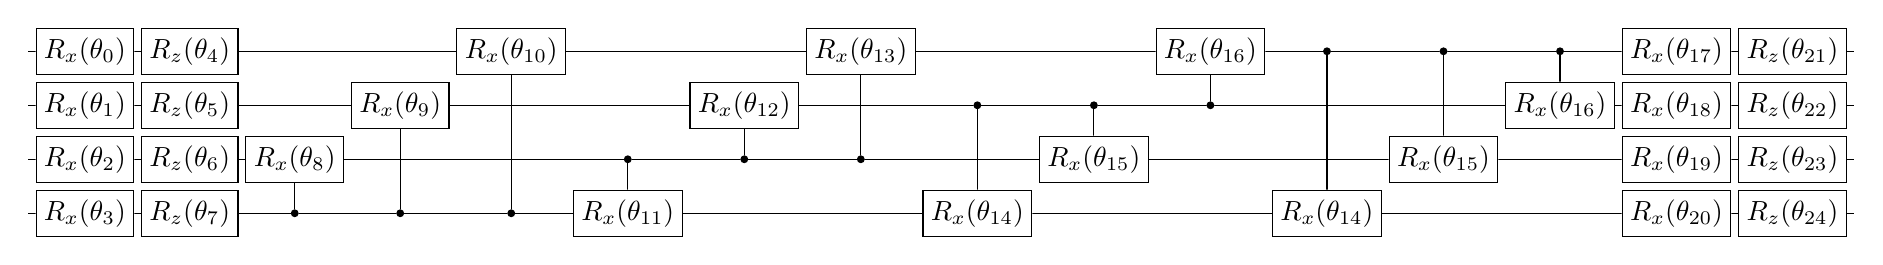
\begin{tikzpicture}
        \begin{yquant}
            qubit {} q[4];
            box {$R_x(\theta_{0})$} q[0];
            box {$R_x(\theta_{1})$} q[1];
            box {$R_x(\theta_{2})$} q[2];
            box {$R_x(\theta_{3})$} q[3];
            box {$R_z(\theta_{4})$} q[0];
            box {$R_z(\theta_{5})$} q[1];
            box {$R_z(\theta_{6})$} q[2];
            box {$R_z(\theta_{7})$} q[3];
            
            box {$R_x(\theta_{8})$} q[2]|q[3];
            box {$R_x(\theta_{9})$} q[1]|q[3];
            box {$R_x(\theta_{10})$} q[0]|q[3];

            box {$R_x(\theta_{11})$} q[3]|q[2];
            box {$R_x(\theta_{12})$} q[1]|q[2];
            box {$R_x(\theta_{13})$} q[0]|q[2];

            box {$R_x(\theta_{14})$} q[3]|q[1];
            box {$R_x(\theta_{15})$} q[2]|q[1];
            box {$R_x(\theta_{16})$} q[0]|q[1];

            box {$R_x(\theta_{14})$} q[3]|q[0];
            box {$R_x(\theta_{15})$} q[2]|q[0];
            box {$R_x(\theta_{16})$} q[1]|q[0];
            align -;
            box {$R_x(\theta_{17})$} q[0];
            box {$R_x(\theta_{18})$} q[1];
            box {$R_x(\theta_{19})$} q[2];
            box {$R_x(\theta_{20})$} q[3];
            box {$R_z(\theta_{21})$} q[0];
            box {$R_z(\theta_{22})$} q[1];
            box {$R_z(\theta_{23})$} q[2];
            box {$R_z(\theta_{24})$} q[3];
            
        \end{yquant}
    \end{tikzpicture}
    }
    \caption{The variational layer of the least expressive VQC proposed by Sim et al.}
    \label{fig:MostExpressive}
\end{figure*}

\subsection{Generalization on different architecture ansatz}
To investigate the dependence of the advantage brought in by AMSGrad on the circuit ansatz, we trained two different VQCs with different circuit ansatzes in the same setting with AMSGrad and the standard SPSA optimizer. Since the difficulty of training the circuit depends strongly on the expressivity, the least and most expressive circuits proposed by Sim et al.~\cite{Sim2019, dragan2022quantum} respectively were chosen to validate the performance of AMSGrad in combination with SPSA-based gradient estimation. \cref{fig:leastExpressive} represents one variational layer of the least expressive circuit, and \cref{fig:MostExpressive} represents one variational layer of the most expressive circuit. Five such layers were repeated in each VQC. The results shown in \cref{tab:expressivity_results} validate that the combination of AMSGrad with SPSA-based gradient estimation yields superior results compared to the standard SPSA method, irrespective of the expressivity of the circuit.

%\textcolor{blue}{To investigate the dependence of the advantage brought in by AMSGrad on the circuit ansatz, we trained two different VQCs with different circuit ansatzes in the same setting with AMSGrad and standard SPSA optimizers. The selected circuits were the least expressive circuit and the most expressive circuit proposed by Sim et al.~\cite{Sim2019, dragan2022quantum}. The reason for this selection is to validate the performance of AMSGrad in combination with SPSA-based gradient estimation over different circuits with different expressiveness, leading to different ease of training and gradient descent to a solution. \cref{fig:leastExpressive} represents one variational layer of the least expressive circuit, and \cref{fig:MostExpressive} represents one variational layer of the most expressive circuit. Five such layers were repeated in each VQC. The results shown in \cref{tab:expressivity_results} validate that the combination of AMSGrad with SPSA-based gradient estimation yields superior results compared to the standard SPSA method, irrespective of the expressivity of the circuit.
%}

\begin{figure}
    \centering
    \resizebox{0.3\linewidth}{!}{%
    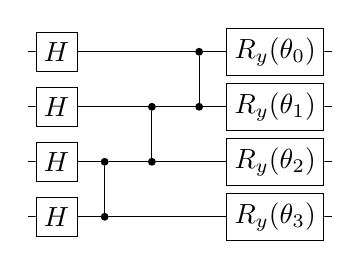
\begin{tikzpicture}
        \begin{yquant}
            qubit {} q[4];
            H q[0];
            H q[1];
            H q[2];
            H q[3];
            zz (q[3, 2]);
            zz (q[2, 1]);
            zz (q[1, 0]);
            align -;
            box {$R_y(\theta_{0})$} q[0];
            box {$R_y(\theta_{1})$} q[1];
            box {$R_y(\theta_{2})$} q[2];
            box {$R_y(\theta_{3})$} q[3];
            
        \end{yquant}
    \end{tikzpicture}
    }
    \caption{The variational layer of the least expressive VQC proposed by Sim et al.}
    \label{fig:leastExpressive}
\end{figure}




\begin{table}[hbtp!]
    \centering
    \caption{Perormance of AMSGrad and SPSA on circuits with different expressivity}

\begin{tabular}{l|l|c|c}
%\hline
Circuit & 
Dataset &
SGD &
%\multicolumn{3}{ c| } {SGD + Momentum}  
AMSGrad  \\
\hline
\multirow{6}{*}{\shortstack[l]{Least \\ Expressive \\ circuit}} 
 & MReg & 0.2166 & 0.0453 \\
 & CCPP & 0.1406 & 0.1142 \\
 & F1 & 0.2839 & 0.1671 \\
 & F2 & 0.5589 & 0.1287 \\
 & F3 & 0.5147 & 0.1652 \\
 \cline{2-4}
 & Norm. Avg. & 1.0000 & 0.4322 \\
 \hline
\multirow{6}{*}{\shortstack[l]{Most \\ Expressive \\ circuit}} 
 & MReg & 0.2192 & 0.0920 \\
 & CCPP & 0.2353 & 0.1236 \\
 & F1 & 0.3099 & 0.2933 \\
 & F2 & 0.5600 & 0.1533 \\
 & F3 & 0.5483 & 0.5149 \\
 \cline{2-4}
 & Norm. Avg. & 1.000 & 0.6208 \\
\end{tabular}

    \label{tab:expressivity_results}
\end{table}
%\input{04_theoretical_consideration}
\section{Conclusion}

This paper proposes an optimization scheme for variational quantum circuits by combining the gradient estimate obtained from simultaneous perturbation stochastic approximation with gradient-based optimizers like SGD, Adam, AMSGrad, or RMSProp. We demonstrate with noiseless simulations on simple regression tasks that using the SPSA-approximated gradient improves both the convergence rate by a factor of three and the final absolute error by a factor of more than two compared to the parameter-shift rule. We further observe that the combined SPSA-AMSGrad optimizer consistently outperforms all other methods, including standard SPSA.

Adam, AMSGrad, and RMSProp clearly outperform SGD for SPSA-inferred gradients when considering shot- and hardware noise. The gap in performance grows to a factor of 1.5 for the full noise model. The performance boost between methods remains the same even when error mitigation addresses the hardware noise.

We conclude that combining the computationally cheap to obtain gradient estimate of SPSA with modern gradient-based optimizers drastically speeds up the training process of VQCs and leads to improved convergence.

% funding is already mentioned on the first page
%The research presented in this paper is supported by the Bavarian Ministry of Economic Affairs, Regional Development and Energy with funds from the Hightech Agenda Bayern.
%%%%%%%%%%%%%%%%%%%%%%%%%%%%%%%%%%%%%%%%%%%%%
%%%%%%%%%%%%%%%%%%%%%%%%%%%%%%%%%%%%%%%%%%%%%
%\let\oldthebibliography=\thebibliography
%\let\endoldthebibliography=\endthebibliography
%\renewenvironment{thebibliography}[1]{%
%\begin{oldthebibliography}{#1}%
%\setlength{\parskip}{1ex plus 1ex minus 0.5ex}%
%\setlength{\itemsep}{6pt}%
%\setstretch{1.0} % ZEILENABSTAND
%}%
%{%
%\end{oldthebibliography}%
%}
\newpage
\bibliographystyle{IEEEtran}
\bibliography{references}

\end{document}
